%!TEX root = ../report.tex
\documentclass[report.tex]{subfiles}
\begin{document}
\chapter{Methodology}

    % How you are planning to test/compare/evaluate your research.
    % Criteria used.

    This chapter describes the methodology on implementing the image matching pipeline used in the project. The methodology outlines the overview of the data and its processing, followed by the implementation of the deep learning and traditional method feature descriptor and feature matching, and concluded with the implementation of clustering. The methodology can be visualized through Figure \ref{fig:methodology} for a quick reference.

    \begin{figure}[!htbp]
        \centering
      % Include your graphic file here
        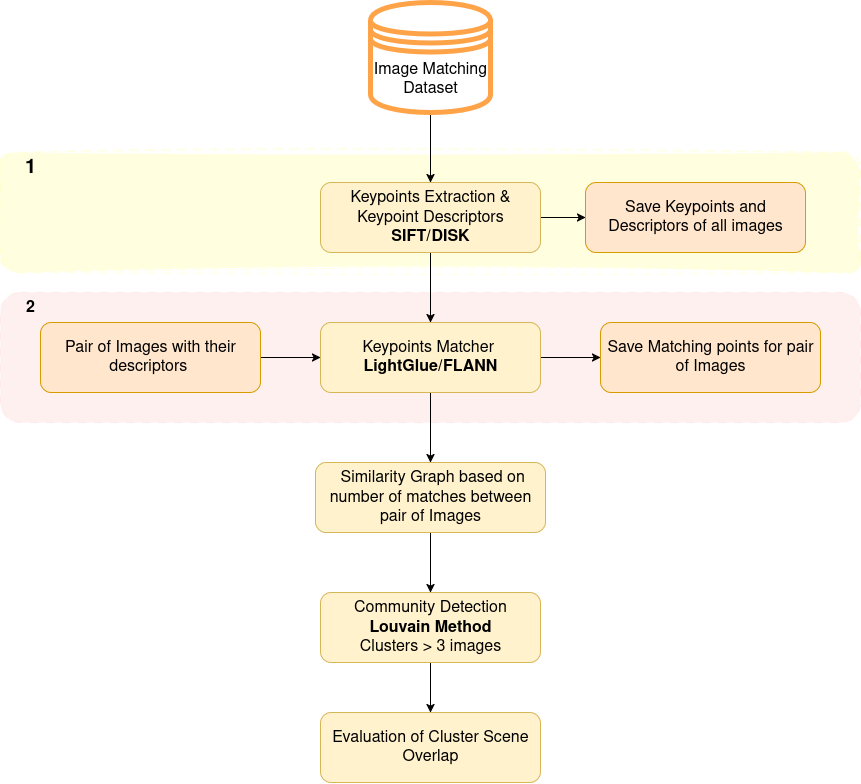
\includegraphics[height=0.65\textwidth]{images/methodology.drawio.png}
        \caption{The figure details the pipeline devised for the problem statement. The pipeline had two independent components that is \textbf{1)} keypoints and keypoint descriptor extraction then saving them for future use, \textbf{2)} Matching pair of images using their descriptors and saving matching points for future use. }
        \label{fig:methodology}
    \end{figure}

    \section{Setup}
    This section presents an overview of the dataset to provide a clearer understanding of its distribution and the preprocessing steps applied prior to its use.
    
    \subsection{Data Collection}
    The dataset for this project was obtain from Kaggle Image Matching Challenge 2025 \cite{image-matching-challenge-2025}. The dataset is divided into 13 datasets with a total of 1.945 images covering following features:
    \begin{itemize}
        \item Dataset name: the unique identifier for the dataset
        \item Scene name: the unique identifier for the scene
        \item Image name: the image name file
        \item Rotation matrix: a 3x3 matrix, flattened into a vector in row-major convention, with values separated by ";"
        \item Translation vector: a 3-D dimensional vector, with values separated by ";"
    \end{itemize}

    \begin{figure}[htbp]
        \centering
        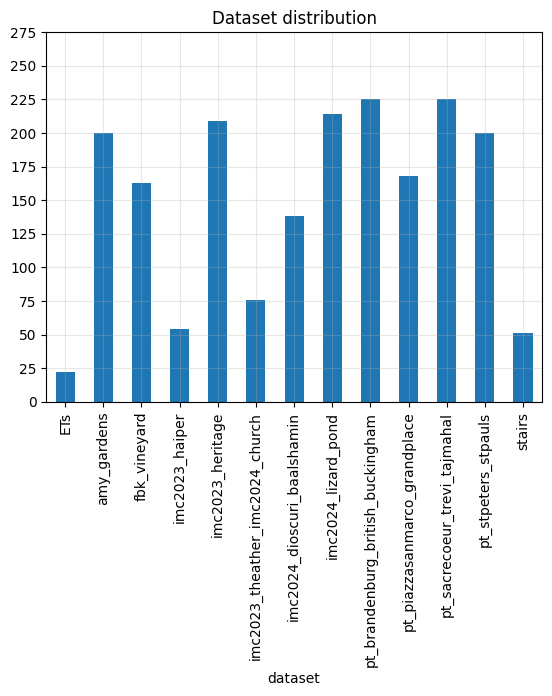
\includegraphics[width = 0.5\textwidth]{images/dataset_distribution.png}
        \caption{Distribution of the dataset}
        \label{fig:dataset-distribution}
    \end{figure}
   

    Figure~\ref{fig:dataset-distribution} illustrates the distribution of each dataset. It shows an imbalance in class distribution between the datasets. The dataset ``ETs" has the lowest number of images, with total below 25 images, while the dataset ``pt\_brandenburg\_british\_buckingham" and ``pt\_sacrecoeur\_trevi\_tajmahal" contain 225 images each.
    
    Each dataset contains between 1 until 4 scenes, with a total of 30 scenes overall. From this 30 scenes there is one scene is defined as an outlier. Figure~\ref{fig:scene-distribution} below is the plot of scene distribution for each dataset.

    \begin{figure}[htbp]
        \centering
        \begin{minipage}[t]{0.48\textwidth}
            \centering
            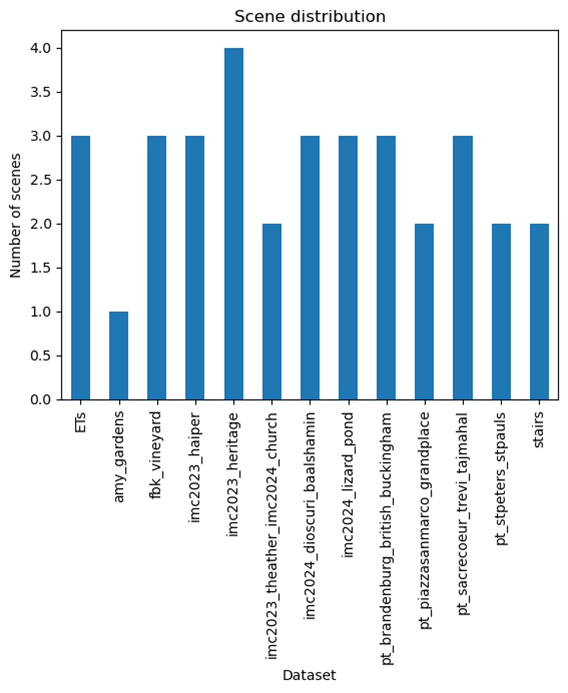
\includegraphics[width=\linewidth, height=7cm]{images/scene_distribution_plog.png}
            \caption{Distribution of scene for each dataset}
            \label{fig:scene-distribution}
        \end{minipage}%
        \hfill
        \begin{minipage}[t]{0.48\textwidth}
            \centering
            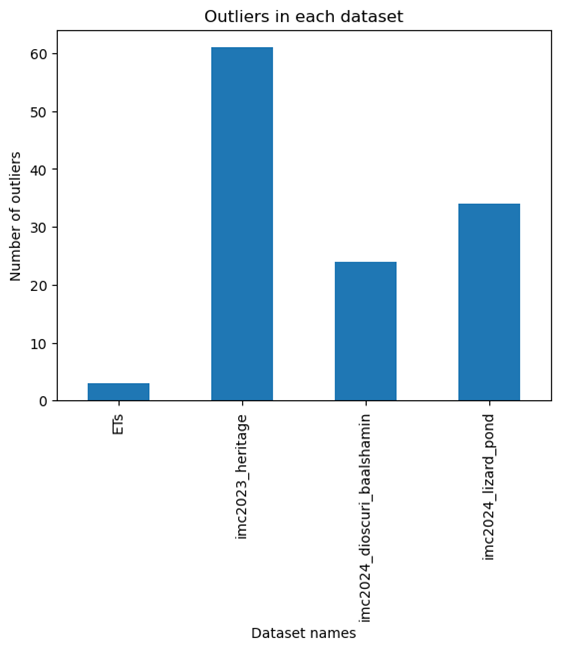
\includegraphics[width=\linewidth, height=7cm]{images/outlier_scene_distribution.png}
            \caption{Distribution of outliers}
            \label{fig:outlier-distribution}
        \end{minipage}
    \end{figure}




    \subsection{Dataset Preprocessing}
    The dataset consists of images with varying size, which poses a challenge in implementing batching in PyTorch, as consistent input size is required for using PyTorch DataLoader. To address this issue, the dataset must be preprocessed prior to model implementation. The preprocessing steps are as follows:

    \begin{enumerate}
        \item Padding
        
        All images with size smaller than 1024 pixels were zero-padded to reach a size of 1024 pixels with custom class \texttt{PadToSize}, whereas images larger than 1024 remain unchanged.
        \item Resize

        All images were resized to a fixed size of 1024 x 1024 pixels to ensure consistency across the dataset and allowed use of batching with the DataLoader.
    \end{enumerate}


    \section{Experimental Design}
    The preprocessed dataset will serve as input for feature extraction, which is performed using two algorithms: SIFT and DISK. The resulting features from both algorithms will then be used for image matching using LightGlue and FLANN. This setup yields in four pipeline combinations: FLANN with SIFT, LightGlue with SIFT, FLANN with DISK, and LightGlue with DISK. Both feature extraction and feature matching will be performed in batches using PyTorch DataLoader, which requires the preprocessing steps to ensure input compatibility. Due to high computational cost, all results from feature descriptor and feature matching will be stored in a \texttt{h5}-file, allowing them to be reused without re-executing the processes.

    For each pipeline, a similarity graph based on its result will be generated, with edges weighted by the number of matches between image pairs. Community detection with Louvain method \cite{Blondel_2008} will then be applied to this graph to identify clusters and detect outliers. The method will create possible connected group within the data based on modularity optimization.

    The identified clusters and outliers will be evaluated against the ground truth scene label, to determine whether images in a given cluster truly belong to the same scene or if multiple scenes are represented within a single cluster. In addition, the evaluation will verify whether the outliers that have been identified are, in fact, outliers according to the ground truth.

    The code implementation is available at \url{https://github.com/arunimaCh29/Image_matching_3d/tree/main}

    \section{Implementation}
    This section describes the implementation of the proposed image matching pipeline, starting with feature descriptor, followed by the feature matching, and concluding with clustering.
    
    \subsection{Feature Descriptor}
    Both SIFT and DISK feature descriptor function will be used from LightGlue library with the \texttt{max\_keypoints} parameter is set to 2048. In order to perform feature extraction, the preprocessed dataset will first be wrapped in PyTorch Dataset. This enables batch processing with PyTorch DataLoader. Minor implementation differences between the two feature descriptors due to different characteristic of each algorithm:

    \begin{itemize}
        \item SIFT

        Since the SIFT function internally relies on OpenCV's implementation, which does not support batch processing, the \texttt{batch\_size} for SIFT's DataLoader is set to 1. The results from each batch are saved into separate files. To consolidate these files, each file is iterated through to determine the maximum number of keypoints, as the results do not guarantee a maximum of 2048 keypoints per image. This approach is necessary because each image contains a different number of descriptors and keypoints, preventing direct use of the DataLoader for image matching. The keypoints and descriptors are padded with zeros while the keypoint scores are padded with \texttt{-inf} to match the size of the maximum keypoints and descriptors. A mask is also created to indicate which entries are actual data and which are padded. After this preprocessing, all files can be merged into a single file.
        \item DISK

        Unlike SIFT, the DISK function supports batch processing, as it is based on a deep learning model. However, its internal implementation attempts to stack keypoints, descriptors, and keypoint scores, which causes issues due to the varying number of keypoints per image. The internal code was modified to perform padding in the same manner as for SIFT. Since most of the output can reach up to 2048 keypoints, padding can be applied directly within each batch. As with SIFT, the results from each batch are saved into separate files and later merged into a single file.
    \end{itemize}
    
    \subsection{Feature Matching}
    Prior to image matching, each image is paired with all other images within the same dataset. The pairings from each dataset are then consolidated into a single CSV file. The feature descriptor outputs for each image in the pairs are added to this list, creating a temporal or pseudo-dataset using custom PyTorch Dataset that will be used for feature matching. There are slight differences in how feature matching is performed within the proposed pipeline:

    \begin{itemize}
        \item FLANN

        For the FLANN implementation, the OpenCV library is used. While batch processing is applied to handle the feature matching, FLANN itself does not support batch operations; therefore, the data within each batch is processed individually. Before matching, the descriptor outputs must be converted into NumPy arrays, as FLANN does not support tensors. Additionally, descriptorts are filtered using the valid mask to retain only valid entries.

        FLANN works by first constructing an index or data structure to organize the data points, for which the kd-tree algorithm is used in this implementation. Subsequently, a k-nearest neighbors (k-NN) search is performed to identify the two nearest neighbors for each query point. The resulting matches are then filtered using the ratio test proposed by Lowe \cite{lowe2004sift} to eliminate false matches.
        
        \item LightGlue

        The LightGlue implementation is based on the LightGlue repository. Although LightGlue supports batch processing, computational limitations necessitate processing each item in a batch individually, similar to the approach used with FLANN. Unlike FLANN, LightGlue natively supports tensors, eliminating the need to preprocess the descriptor output data types. The matching process is executed using the \texttt{matcher} function, which takes a dictionary containing the descriptor data of the two images.
    \end{itemize}

    The results of feature matching from each matcher are stored in separate files after every 10 batches and subsequently merged into a single CSV file, which is then used for the clustering process.
    \subsection{Clustering}
We build a weighted image-similarity graph per dataset, where nodes are images; edges connect image pairs with verified matches and edge weights equal the number of geometrically consistent correspondences.

Given tentative correspondences \((\mathbf{x}_i \leftrightarrow \mathbf{x}'_i)\), we estimate a fundamental matrix with RANSAC and keep only inliers (mask) to compute edge weights.
This suppresses false matches and preserves structure-indicative links.

We cluster via Louvain modularity optimization on the weighted graph to obtain communities \(\mathcal{C} = \{C_k\}\).
It is scalable, uses weights natively, and is non-parametric (no need to predefine \(K\)).

Let \(s_k = |C_k|\) and \(\alpha = \max\{3, \mathrm{median}(\{s_k\})\}\).
Communities with \(s_k \ge \alpha\) are reported as clusters; otherwise they are marked as outliers.

\textbf{Advantages:}
\begin{itemize}
  \item \textbf{Robustness:} RANSAC enforces geometric consistency, reducing spurious edges.
  \item \textbf{Scalability:} Louvain handles large, sparse, weighted graphs efficiently.
  \item \textbf{Parameter-light:} No preset \(K\); the size threshold \(\alpha\) adapts to data.
  \item \textbf{Interpretability:} Graph structure and community assignments are easily inspected; labels can display scene and image id.
  \item \textbf{Flexibility:} Works across matchers/descriptors (e.g., SIFT, DISK, LightGlue) by plugging into edge weights.
\end{itemize}

\end{document}
